\documentclass{beamer}\usepackage[]{graphicx}\usepackage[]{color}
%% maxwidth is the original width if it is less than linewidth
%% otherwise use linewidth (to make sure the graphics do not exceed the margin)
\makeatletter
\def\maxwidth{ %
  \ifdim\Gin@nat@width>\linewidth
    \linewidth
  \else
    \Gin@nat@width
  \fi
}
\makeatother

\definecolor{fgcolor}{rgb}{0.345, 0.345, 0.345}
\newcommand{\hlnum}[1]{\textcolor[rgb]{0.686,0.059,0.569}{#1}}%
\newcommand{\hlstr}[1]{\textcolor[rgb]{0.192,0.494,0.8}{#1}}%
\newcommand{\hlcom}[1]{\textcolor[rgb]{0.678,0.584,0.686}{\textit{#1}}}%
\newcommand{\hlopt}[1]{\textcolor[rgb]{0,0,0}{#1}}%
\newcommand{\hlstd}[1]{\textcolor[rgb]{0.345,0.345,0.345}{#1}}%
\newcommand{\hlkwa}[1]{\textcolor[rgb]{0.161,0.373,0.58}{\textbf{#1}}}%
\newcommand{\hlkwb}[1]{\textcolor[rgb]{0.69,0.353,0.396}{#1}}%
\newcommand{\hlkwc}[1]{\textcolor[rgb]{0.333,0.667,0.333}{#1}}%
\newcommand{\hlkwd}[1]{\textcolor[rgb]{0.737,0.353,0.396}{\textbf{#1}}}%
\let\hlipl\hlkwb

\usepackage{framed}
\makeatletter
\newenvironment{kframe}{%
 \def\at@end@of@kframe{}%
 \ifinner\ifhmode%
  \def\at@end@of@kframe{\end{minipage}}%
  \begin{minipage}{\columnwidth}%
 \fi\fi%
 \def\FrameCommand##1{\hskip\@totalleftmargin \hskip-\fboxsep
 \colorbox{shadecolor}{##1}\hskip-\fboxsep
     % There is no \\@totalrightmargin, so:
     \hskip-\linewidth \hskip-\@totalleftmargin \hskip\columnwidth}%
 \MakeFramed {\advance\hsize-\width
   \@totalleftmargin\z@ \linewidth\hsize
   \@setminipage}}%
 {\par\unskip\endMakeFramed%
 \at@end@of@kframe}
\makeatother

\definecolor{shadecolor}{rgb}{.97, .97, .97}
\definecolor{messagecolor}{rgb}{0, 0, 0}
\definecolor{warningcolor}{rgb}{1, 0, 1}
\definecolor{errorcolor}{rgb}{1, 0, 0}
\newenvironment{knitrout}{}{} % an empty environment to be redefined in TeX

\usepackage{alltt}
\usepackage{../371g-slides}
% Uncomment these lines to print notes pages
% \pgfpagesuselayout{4 on 1}[letterpaper,border shrink=5mm,landscape]
% \setbeameroption{show only notes}
\title{Probability Review 1}
\subtitle{Lecture 2}
\author{STA 371G}
\IfFileExists{upquote.sty}{\usepackage{upquote}}{}
\begin{document}
  
  

  \frame{\maketitle}

  % Show outline at beginning of each section
  \AtBeginSection[]{ 
    \begin{frame}<beamer>
      \tableofcontents[currentsection]
    \end{frame}
  }

  %%%%%%% Slides start here %%%%%%%

   \begin{darkframes}
  

    \begin{frame}[label=lists]{Probability Theory}
      \framesubtitle{The Concept of Probability}
      
      What is common among the following?
      
      \begin{itemize}
      	\item Outcome of rolling a die
      	\item S\&P500 index at the and of January
      	\item Number of iPhone 7s to be sold over the next year
      	\item Number of unique visitors to Amazon.com over the next week
      	\item Lifetime of your MacBook Air
      \end{itemize}
      
      We cannot predict any of these with certainty. 
      
      Yet, we can model them using \alert{probability theory} and study the values they might take, associated probabilities etc.
      
     \end{frame}    


    \begin{frame}[label=lists]{Probability Theory}
		\framesubtitle{Definitions}    
		\begin{definition}
       		A \alert{random variable} expresses the outcome of a \alert{random experiment} as a number. It is denoted by an uppercase letter.
      	\end{definition} 	
      	
      		\begin{itemize}
      			\item Random experiment $\rightarrow$ Rolling a die
      			\item Random variable $\rightarrow$ $X:$ The outcome when a die is rolled
				\item Random variable $\rightarrow$ $$ Y : \begin{cases}
        					1, \qquad \text{if outcome is odd number,}  \\
        					2, \qquad \text{if outcome is even number}  
        		            \end{cases}
        		      $$ 
        	\end{itemize}	
	
	%Use lowercase letter to denote a particular realization of a random variable, e.g., $x=6$.
				
    \end{frame}
    
       
    

    \begin{frame}[label=lists]{Probability Theory}
		\framesubtitle{Definitions}    
      	
      	\begin{definition}
       		A \alert{discrete random variable} is a random variable with a finite (or countably infinite) range. 
       		
       		A \alert{continuous random variable} is a random variable with an interval (either finite or infinite) of real numbers for its range.
      	\end{definition}
    
    
    	\begin{exampleblock}{Examples}
      		\begin{itemize}

				\item $X:$ Number of stocks on NYSE whose price change today (discrete)
				\item $Y:$ Average price change of the stocks on NYSE (continuous)

			\end{itemize}
        \end{exampleblock}
  
	\end{frame}  
	
	
	
   \begin{frame}[label=lists]{Probability Theory}
		\framesubtitle{Exercise}    
      	Discrete or continuous?
      		\begin{itemize}
				
				\item Number of iPhone 7s to be sold over the next year
				\item Lifetime of your MacBook Air
				\item Number of unique visitors to Amazon.com over the next week
      			\item S\&P500 index at the and of January % This could be interpreted both discrete or continuous
    
			\end{itemize}
	\end{frame} 
	
	
	
	\begin{frame}[label=lists]{Probability Theory}
		\framesubtitle{Definitions}    
		
      	\begin{definition}
       		\alert{Probability} is the measure of the likelihood that a particular outcome (or set of outcomes) will be observed. \newline
       		
       		Probability is a number always between 0 and 1. \newline
       		
       		0 implies impossibility, 1 implies certainty.
      	\end{definition}
    
    
    	\begin{exampleblock}{Examples}
      		\begin{itemize}

				\item $X:$ S\&P500 at the end of 2017, $P(X>2270) = 0.85$ % It was 1/18 price. We are optimistic about Trump
				\item $Y:$ Lifetime of your MacBook, $ P(Y>15\text{ years})  = 0.05$

			\end{itemize}
        \end{exampleblock}
  
	\end{frame}  	
	
	
  
  
  
  
  
	\begin{frame}[label=lists]{Probability Distributions}
	%	\framesubtitle{How to express probabilities} 
	
		So, we have defined a random variable. How do we know what the probabilities are? \newline
		
		For example, what is the probability that your MacBook will break down after 5 years but before 7 years? That is, $P(5<X<7)=?$\newline
  
		
      	\begin{definition}
       		The \alert{probability distribution} of a random variable $X$ is a description of the probabilities associated with the possible values of $X$. 
			\newline       		
       		
       		Discrete random variable $\rightarrow$ Probability Mass Function (p.m.f.)
       		
       		Continuous random variable $\rightarrow$ Probability Density Function (p.d.f.)

      	\end{definition}
    
    
		
  
	\end{frame}  	
	  
  
  




	\begin{frame}[label=lists]{Probability Distributions}
		\framesubtitle{Discrete Random Variables} 
	
		\begin{exampleblock}{Example}
			$X$: The outcome when you roll $n$-sided fair die.
			
			Since this is a fair die, the corresponding probability mass function:
			
			$$ f(x) = 
			\begin{cases}
				\frac{1}{n} \qquad x= 1,\ldots,n, \\
				0 \qquad   \text{otherwise.}
			\end{cases}
			$$
        \end{exampleblock}
        
       
        \begin{itemize}
        	\item $f(2)=P(X=2)$, which is the probability of observing a ``2.'' This interpretation will not hold for continuous random variables.
        	
        	\item Sum of probabilities is always 1. ($n \times \frac{1}{n}$). 
    		
    		\item This is an example of \alert{Discrete Uniform Distribution}.    	
	        	
        \end{itemize} 
	\end{frame}







	\begin{frame}[label=lists]{Probability Distributions}
		\framesubtitle{Continous Random Variables} 
	
		\begin{exampleblock}{Example}
		$Y:$ Lifetime of your MacBook (in years) \newline
		
		Let's assume $Y$ has a \alert{Continuous Uniform Distribution} with a maximum of 20 years. Its probability distribution is then given by the following probability density function: \newline
		
		$$ f(y) = 
			\begin{cases}
				\frac{1}{20} \qquad 0 \leq y \leq 20, \\
				0 \qquad   \text{otherwise.}
			\end{cases}
		$$
		
		What is $P(Y=5)=?$ or $P(Y=5.5)=?$ or $P(Y=5.551234123)=?$ \newline
		They are all 0.
		
		
		\end{exampleblock}
			
	\end{frame}





	\begin{frame}[label=lists]{Probability Distributions}
		\framesubtitle{Continous Random Variables} 
	
		\begin{alertblock}{Warning!}
        For a continuous random variable, $P(Y=a)$ is always zero, regardless of $a$. \newline
      \end{alertblock} 
       %\quad \newline
      
      For this reason, for continuous random variables we ask questions like ``$P(a \leq Y \leq b)=?$'' \newline
      
      And we take integrals to find such probabilities.
			
	\end{frame}


	\begin{frame}[label=lists]{Probability Distributions}
		\framesubtitle{Continous Random Variables} 

		\begin{exampleblock}{Example}
		$Y:$ Lifetime of your MacBook (in years) \newline
		
		$$ f(y) = 
			\begin{cases}
				\frac{1}{20} \qquad 0 \leq y \leq 20, \\
				0 \qquad   \text{otherwise.}
			\end{cases}
		$$
		
		What is $P(5<Y<7)=?$ 
		
		$$
			P(5<Y<7) = \int_5^7 \frac{1}{20} dy = \frac{y}{20} |_5^7 = \frac{7}{20} - \frac{5}{20} =  \frac{1}{10}
		$$
		
		
		\end{exampleblock}
		
		In general, \alert{$P(a \leq Y \leq b) = \int_a^b f(y)dy$}.
				
	\end{frame}




	\begin{frame}[label=lists]{Probability Distributions}
		\begin{figure} 
			\centering
			\scalebox{1}{ 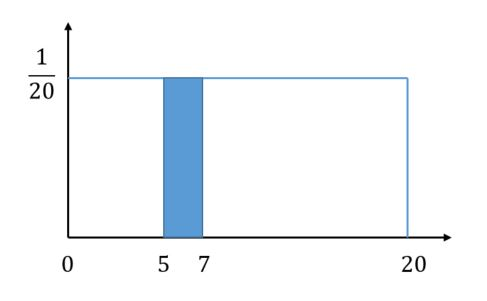
\includegraphics{unif_ex2.jpg} }
			\setlength\fboxsep{0pt}
			\setlength\fboxrule{0.5pt}
		\end{figure} 


				
	\end{frame}
	
	
	
	\begin{frame}[label=lists]{Mean, Variance and Standard Deviation}
		%\framesubtitle{Mean (Expected Value) of a Random Variable} 
		
		\begin{definition}
			\alert{Mean} or \alert{Expected Value} of a random variable $X$ is a measure of the center of its probability distribution. It is a weighted average of all possible values $X$ can take, where the weights are the corresponding probabilities. 
		\end{definition}
		
		\begin{columns}[onlytextwidth]
        \column{.5\textwidth}
        	Discrete random variable $X$
        	$$
				\mu_X = E[X] = \sum_x x f(x)	        	
        	$$
        	
        \column{.5\textwidth}
        	Continuous random variable $Y$
        	$$
				\mu_Y = E[Y] = \int_y y f(y) dy	        	
        	$$
        	        
        \end{columns}


				
	\end{frame}





	\begin{frame}[label=lists]{Mean, Variance and Standard Deviation}
		%\framesubtitle{Mean (Expected Value) of a Random Variable} 
		
		\begin{definition}
			\alert{Variance} of a random variable $X$ is a measure of the dispersion, or variability in its distribution. \alert{Standard Deviation} of $X$ is the square root of its variance.
		\end{definition}
		
        	Discrete random variable $X$
        	$$
				\sigma^2_X = Var(X) = E[(X-\mu_X)^2] = \sum_x (x-\mu_x)^2 f(x)	        	
        	$$
        	
        	Continuous random variable $Y$
        	$$
				\sigma^2_Y = Var(Y) = E[(Y-\mu_Y)^2] = \int_y (y-\mu_y)^2 f(y)dy	        	
        	$$
   			
	\end{frame}





	\begin{frame}[label=lists]{Law of Large Numbers}
		%\framesubtitle{Mean (Expected Value) of a Random Variable} 
		
		\begin{definition}
			For a random variable $X$, the average of $X_1, X_2,\ldots,X_n$ gets very close to the expected value of $X$ ($E[X]$) for large $n$.
		\end{definition}
		\begin{exampleblock}{Example}
			A die is rolled $n=4$ times: $x_1=4, x_2=6, x_3=1, x_4=1$. The average is
			$$
				\frac{x_1 + x_2 + x_3 + x_4}{4} = \frac{4+6+1+1}{4}=3
			$$
		\end{exampleblock}
		
		For large $n$, the average will be around 3.5; because $E[X]=3.5$.
   			
	\end{frame}
	
	
	 
	
	
	
	\defverbatim[colored]\rollRie{
      \begin{lstlisting}[language=R,tabsize=2]
# Generate a random number in [0,1]
runif(1) 
# Generate a random number in [1,7]
runif(1, min=1, max=7)
# Floor it down to simulate a die
floor(runif(1, min=1, max=7))
# Simulate 3 dice
floor(runif(3, min=1, max=7))
# Take the average	
mean(floor(runif(3, min=1, max=7)))
# Let's increase the number of dice
mean(floor(runif(10, min=1, max=7)))

    \end{lstlisting}}	
	
	\begin{frame}[label=lists]{Law of Large Numbers}
		\framesubtitle{R Exercise} 
		Go to R Studio...
		
		\rollRie
   			
	\end{frame}




	\begin{frame}[label=lists]{Normal Distribution a.k.a. the Bell Curve}
		%#\framesubtitle{R Exercise} 
		A very common continuous probability distribution. 

		The mean and variance together uniquely define the distribution: $N(\mu,\sigma^2)$		
		
		
		\begin{figure} 
			\centering
			\scalebox{0.8}{ 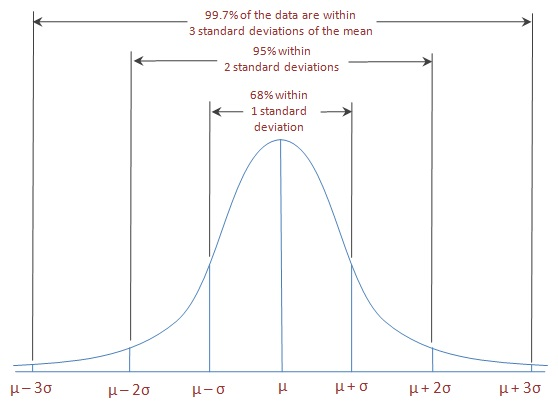
\includegraphics{normal.jpg} }
			\setlength\fboxsep{0pt}
			\setlength\fboxrule{0.5pt}
		\end{figure}
		
		
   			
	\end{frame}
	
	
	
	
	
	\begin{frame}[label=lists]{Central Limit Theorem}
		%\framesubtitle{R Exercise} 
		\begin{definition}
			The average of large number of independent random variables will be approximately normally distributed.
		\end{definition}		
		
		\begin{exampleblock}{Example}
			$$
				\text{a student's exam grade} = \frac{  \text{preparedness} + \text{focus} + \text{IQ} + \ldots  }{ \text{\# of factors}}
			$$
		\end{exampleblock}
		
		Distribution of the exam grades then tend to be normal...

   			
	\end{frame}	
	
	
	
	
	
	
	
	\defverbatim[colored]\housePrices{
      \begin{lstlisting}[language=R,tabsize=2]
# Simulating a zip code with 3 houses
runif(3, min=100, max=400)
# Repeat this for 5 zip codes.
house_prices <- t(replicate(5, runif(3, min=100, max=400) ))
# Find the average house price in each zip code
avg_house_prices <- rowMeans(house_prices)
# See what you got
hist(avg_house_prices)
# Increase n and z and try again!
    \end{lstlisting}}		
	
	\begin{frame}[label=lists]{Central Limit Theorem}
		\framesubtitle{R Exercise} 
		 $X$ : The price of a house. Assume $X$ is uniform in $[100,400]$ (\$K).
		 
		 $Y$ : Average house price in a zip code
		 
		 We will simulate $z$ number of zip codes, each containing $n$ houses.		 	
		
		
		\housePrices
   			
	\end{frame}	










\end{darkframes}
  
  
  

\end{document}

